\chapter{E-Mails des Auftraggebers}
\begin{figure}[ht!]
    \centering
    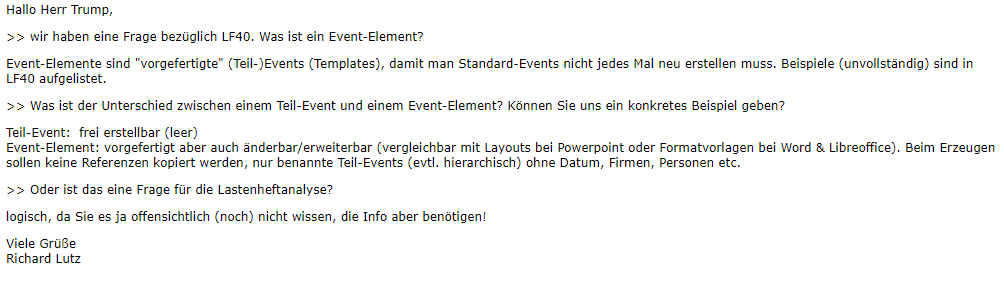
\includegraphics[width=1.0\textwidth]{Bilder/mail_eventelemente.png}
    \caption{Mail des Auftraggebers}
    \label{fig:email:eventelemente}
\end{figure}
In \autoref{fig:email:eventelemente} ist der Screenshot einer Mail des Auftraggebers zu sehen, in welcher die Bedeutung des Begriffes \enquote{Eventelement} im Lastenheft genauer geklärt wird.